\documentclass{article}
\usepackage{amsfonts}
\usepackage{graphicx}
\usepackage{enumitem}
\usepackage{amsmath}
\usepackage{float}
\usepackage{tfrupee}
\usepackage{gensymb}
\begin{document}
\begin{enumerate}
\item find the distance of a point $P(x,y)$ from the origin.
\item what is the value of $(\cos^2{67^\circ}$-$\sin^2{23^\circ})$ ?
\item Given $\Delta ABC ~ \Delta PQR$,if $\frac{AB}{PQ}$=$\frac{1}{3}$ , then find $\frac {ar \Delta ABC}{ar \Delta PQR}$ .
\item Find the ratio in which $P(4,m)$ divides the line segment joining the points $A(2,3)$ and $B(6,-3)$.Hence find m .
\item Two different dice are tossed together.Find the probability:
	\begin{enumerate}[label=\roman*)]
		\item of getting a doublet
		\item of getting a sum $10$,of the numbers on the two dice .
	\end{enumerate}
\item An integer is chosen at random between $1$ and $100$.Find the probability that it is:
	\begin{enumerate}[label=\roman*)]
		\item divisible by $8$ .
		\item not divisible by $8$ .
	\end{enumerate}
\item Find $HCF$ and $LCM$ of $404$ and $96$ and verify that $HCF \times LCM =$ product of two given numbers .
\item Find the zeros of the polynomial$(2x^4-9x^3+3x-1)$.If two of its zeros are $(2+\sqrt+3)$ and $(2-\sqrt+3)$ .
\item If $ A(-2,1)$,$ B(a,0)$,$ C(4,b)$ and $ D(1,2)$ are the vertices of a parallelogram $ABCD$,find the values of a and b.Hence find the length of its side.
\item If $  A(-5,7)$,$ B(-4,-5)$,$ C(-1,-6)$ and $ D(4,5)$ are the vertices of a quadrilateral,find the are of the quadrilateral $ABCD$.
\item If $4\tan\theta=3$,evaluate$(\frac {4\sin\theta-\cos\theta+1} {4\sin\theta+\cos\theta-1})$.
\item If $( \tan 2A)$ = $\cot(A - 18\degree)$  where $(2A)$is an acute angle, find the value of $(A)$.
\item Find the area of the shaded region in fig 2,where areas drawn with centers $A$ ,$B$ ,$C$ and $D$ intersect in pair at mid-points.$P$, $Q$, $R$ and S of the sides $AB$,$BC$,$CD$ and $DA$ respectively of a square $ABCD$ of side $12cm$.$[use \pi=3.14]$ .
			\begin{figure}[H]
				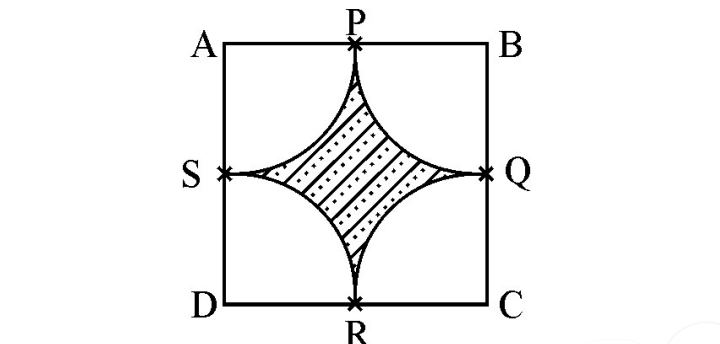
\includegraphics [width=\columnwidth]{./IMG3.jpg}
				\label{fig;fig2}
				\caption{square}
			\end{figure}
\item Prove that $\frac{\sin A - 2\sin^3 A}{2\cos^3 A - \cos A} = \tan A$.
\item The diameters of the lower and upper ends of a bucket in the form of a frustum of a cone are $10cm$ and $30cm$ respectively.If its height is $24cm$,find:
                \begin{enumerate}[label=\roman*)]
                        \item The area of the meta sheet used to make the bucket.
                        \item Why we should avoid the bucket made by ordinary plastic? $[use\pi=3.14]$
		\end{enumerate}
\item As observed from the top of a $100m$ high light house from the sea-level,the angles of depression of two ships are $30\degree$ and $45\degree$.If one ship is exactly behind the other on the same side of the light house,find the distance between the two ships.$[use \sqrt3=1.732]$.
\item The mean of the following distribution is $18$.Find the frequency f of the c
lass $19-21$.
                \begin{table}[htb]                                          
                        \resizebox {\columnwidth}{!}{
                                \begin{tabular}{|c|c|c|c|c|c|c|c|c|}                                              \hline
                        \textbf{class} & 11-13 & 13-15 & 15-17 & 17-19 & 19-21 & 21-23 & 23-25 \\                                                                                                           \hline
                        \textbf{frequency} & 3 & 6 & 9 & 13 & f & 5 & 4 \\ \hline                                         \end{tabular}
                        }
                \end{table}
\item The following distribution gives the daily income of $50$ workers of a factory:
\begin{table}[htb]
	\resizebox {\columnwidth}{!}{
		\begin{tabular}{|c|c|c|c|c|c|c|}
			\hline
			\textbf{DailyIncome$(in\rupee)$} & 100-120 & 120-140 & 140-160 & 160-180 & 180-200 \\
			\hline
			\textbf{Number of workers} & 12 & 14 & 8 & 6 & 10 & \\ 
			\hline
		\end{tabular}
	}
	\end{table}\\
\item Convert the distrubution above to a less than type cumulative frequency distribution and draw its ogive.
	\end{enumerate}
	\end{document}


	
		
